\chapter{AbaaS - Atomic Broadcast as a Service}

% **************************** Define Graphics Path **************************
\ifpdf
    \graphicspath{{Chapter3-TxService/Figs/Raster/}{Chapter3-TxService/Figs/PDF/}{Chapter3-TxService/Figs/}}
\else
    \graphicspath{{Chapter3-TxService/Figs/Vector/}{Chapter3-TxService/Figs/}}
\fi

%Introduction

This chapter introduces the concept of providing \emph{abcast} messaging as a service to members of a cluster.

First we describe the rational behind \textsf{Abaas}, then we explore the requirements of such a service and the challenges involves in meeting them.  This is followed by the introduction of the \textsf{ABService} protocol that is used to implement \textsf{AbaaS}.  We then explain the methodology used to evaluate \textsf{ABService}, before presenting the results of our performance evaluation.  Finally, we discuss the limitations of existing \emph{abcast} protocols in the context of \textsf{AbaaS}, and propose the need for a new non-blocking \emph{abcast} solution.  

\section{Rational}
Total order commit protocols can be utilised by distributed systems to coordinate transactions without the use of locks.  Reducing the abort rate of transactions when contention is high, as system deadlocks do not occur when distributed locks are not present.  Therefore, total order commit protocols can aid scalability as they improve transaction throughput \citep{Ruivo:2011:ETO:2120967.2121604}.  

The limiting factor of total order commit protocols is the underlying \emph{abcast} protocol used to provide atomic guarantees on message delivery.  The TOA protocol currently utilised by Infinispan, does not scale well as the number of destinations $N$ increase, as $N->1$ communication is expensive ($\S$ \ref{ssec:TOA_limations}).  Similarly, other GM protocols such as Newtop \citep{Ezhilchelvan:1995:NFG:876885.880005}, exasperate the problem, as the number of messages required to perform an \emph{abcast} increases dramatically as $N$ increases.  Finally, Quorum based protocols provide even less scalability, then GM based protocols, as their inability to \emph{abcast} messages to disjoint sets of nodes typically requires all nodes in the cluster to participate in an \emph{abcast}.  

Regardless of the \emph{abcast} protocol used, $N->1$ communication is inherently unscalable.  Therefore, we propose that reaching a consensus on \emph{abcast} ordering should not be conducted between a transaction coordinator $Tx.c$ and its participating Infinispan nodes $Tx.dst$, but instead atomic ordering should be provided by an independent coordination service and consumed by $Tx.c$.  It is then the responsibility of $Tx.c$ to coordinate $Tx$, with $Tx.dst$, using the ordering provided by this service.  We call this system model Atomic Broadcast as a Service (\textsf{AbaaS}), and refer to the existing Infinispan approach as \emph{peer-to-peer} (P2P).  

Utilising \textsf{AbaaS} decouples message broadcasting and message ordering, by restricting the number of nodes conducting \emph{abcast} messages to the nodes providing the service; known as \emph{service} nodes, or simply $s$-nodes, and denoted as $N_s$; Infinispan nodes are known as \emph{client} nodes, or simply $c$-nodes, and denoted as $N_c$.  This decoupling means that regardless of $\left\vert Tx.dst \right\vert$, the number of nodes that execute a \emph{abcast} protocol, to obtain a total order for $Tx$, will always be equal to $\left\vert s\text{-nodes}\right\vert$.  Furthermore, restricting \emph{abcast}s to $s$-nodes means that, for all \emph{abcast}s, $m.dst$ will be the same, therefore \emph{abcast}s always occur between a single destination set, which increases performance ($\S$ \ref{ssec:single_destination_set}) and enables certain optimisations to be made ($\S$ \ref{ssec:abaas_optimisations}).  

For a totally ordered 1PC transaction in Infinispan, \textsf{AbsaaS} works as follows: Once $Tx_i.c$ has completed its local execution of $Tx_i$, it is ready to \emph{abcast} a $prepare(Tx_i)$ message $m$.  $Tx_i.c$ selects some $s$-node and forwards $m$ with $m_i.dst = Tx_i.dst$ to the selected $s$-node, say, $N_s$, for \emph{abcast}ing $m$ to $m_i.dst$. $N_s$ actually \emph{abcast}s $m_i$ \emph{only} to other $s$-nodes, which leads to all operative $s$-nodes delivering $m_i$. When $N_s$ delivers $m_i$, it returns $m_i$ to $Tx_i.c$, who then disseminates $m_i$ to every node $d$ indicated in $m_i.dst$ together with two types of order related information: $m_i.ts$ agreed by $s$-nodes and the \emph{immediate} predecessor. The latter is the identity of $m_j$ whose delivery must \emph{precede} \emph{immediately} before delivery of $m_i$. More precisely, $d \in m_j.dst$, $d$ must not deliver $m_i$ until it delivers $m_j$, and no \emph{abcast} other than $m_i$ must be delivered immediately after $m_j$ is delivered.

Note that the immediate predecessor of $m_i$ with respect to \emph{all} \emph{abcast}s directed at a given $d$ - not just those that originate from $Tx_i.c$ nor just those that are handled only by $N_s$. Thus, it is specific to each $d$ and ensures that delivery at every $d$ is as per the finalized $m.ts$. To illustrate this, let $Tx_i.c$ submit $m_i$ to $N_s$, $Tx_j.c$ submit $m_j$ to $N_{s'}$ and $d \in m_i.dst \cap m_j.dst $. Say, $s$-nodes order $m_j$ before $m_i$. If $d$ receives $m_i$ before $m_j$, it will not deliver $m_i$ until it delivers $m_j$.


	\subsection{AbaaS Optimisations}\label{ssec:abaas_optimisations}
	The \textsf{Abaas} model allows for two key optimisations that are not possible when \emph{abcast}ing occurs directly between $N_c$ nodes: \emph{Message Bundling} and \emph{Acknowledgement Piggybacking}.  
	
	\paragraph{Message Bundling} \hspace{0pt} \\
	As the number of concurrent transactions between $c$-nodes increases, the total number of \emph{abcast}s required also increases.  When utilising \emph{abcast}s between $c$-nodes to coordinate the transactions, typically it is not possible to bundle multiple \emph{abcast} messages $<m_i, m_j>$, into a single \emph{abcast}, $m$, due to the high probability of $m_i.dst \neq m_j.dst$.  Of course it is possible to implement a bundling strategy that is utilised only when $m_i.dst = m_j.dst$, however in a system such as Infinispan the performance improvements provided by such a strategy are negligible; as the wide distribution of key/value pairs significantly reduces the probability of two \emph{abcast}s having the same destination set.  
	
	However, when utilising \textsf{AbaaS} it is possible for all \emph{abcast} requests received from $c$-nodes to be bundled at a receiving $s$-node, regardless of their destination set.  This is because $s$-nodes only send \emph{abcast}s to other $s$-nodes, therefore the destination set is the same for all $c$-node requests.  
	
	The ability to bundle multiple \emph{abcast} requests into a single \emph{abcast} can significantly reduce the total amount of network traffic, therefore improving the request capacity and scalability of a \emph{AbaaS} service.  Furthermore, message bundling does not compromise performance when the number of requests to the service are low, as it does not require any additional communication steps or intensive computation.  
	
	\paragraph{Acknowledgement Piggybacking} \hspace{0pt} \\
	As all $s$-nodes send \emph{abcast}s to all other $s$-nodes, and hence, always have the same destination set, it is possible for message acknowledgements to be piggybacked, therefore enabling \emph{abcast}s to be completed with just a single dedicated broadcast ($\S$ \ref{ssec:newtop}).  This optimisation is ideal for a \textsf{AbaaS} service: as all nodes in the service must handle $c$-node requests, thus ensuring that each $s$-node frequently sends \emph{abcast}s containing piggybacked acknowledgements; and, it aids scalability as it reduces the number of messages sent over the network. 
	
	\subsection{AbaaS Deployment Possibilities}
	Implementing transaction ordering as a dedicated service, provides distinct advantages for system administrators.  When utilising the P2P \emph{abcast} approach, administrators would typically want to run Infinispan over a cluster of nodes utilising a homogeneous hardware specification to ensure that Infinispan's performance would not be hamstrung by a lesser machine.  In an environment where low-latency and high-capacity in-memory database is desired, this would require a large number of expensive machines.  
	
	However, when AbaaS is utilised, it is possible to improve the performance of the entire cluster, simply by upgrading the $s$-nodes used to provide the \emph{AbaaS} service.  For example, consider a cluster consisting of 50 $c$-nodes, and 3 $s$-nodes, instead of upgrading all 50 $c$-nodes it is possible to improve transaction latency and throughput by upgrading the hardware of the 3 $s$-nodes.  
	
\section{AbaaS System Requirements}
The \textsf{AbaaS} model consists of two distinct entities: $s$-nodes and $c$-nodes.  This section will explore the requirements that need to be met in order for the \textsf{AbaaS} model to be effective.  We consider requirements from the perspective of both clients, $c$-nodes, and the ordering service, $s$-nodes.

	\paragraph{Client Requirements} \hspace{0pt}
	\begin{itemize}
		\item [\textbf{CR1}] Clients must be able to send \emph{abcast}s to multiple destination sets that may overlap.
		
		\item [\textbf{CR2}] The service must provide a consistent total order $m.ts$ on messages irrespective of the $s$-node handling a clients request, or the $c$-node from which the clients request originated.  
		
		\item [\textbf{CR3}] Client nodes must be informed of $m_i$ when handling $m_j$, if $m_i.dst \cap m_j.dst$ to ensure that $m_i$ is not missed by a $c$-node in $m_i.dst$.  
	\end{itemize}
	
	\paragraph{Service Requirements} \hspace{0pt}
	\begin{itemize}
		\item [\textbf{S1}] The service must be fault-tolerant ($s\text{-nodes} > 1$), and aim to be highly available.  
		
		\item [\textbf{S2}] Service nodes must process client requests in the exact same order to maintain a consistent state between all $s$-nodes.  This prevents a $c$-node from receiving conflicting ordering data, for example two distinct $m$ being allocated the same global timestamp.  
		
		\item [\textbf{S3}] All $s$-nodes should be able to handle client requests, to allow for high availability and to prevent a single $s$-node becoming a performance bottleneck.
	\end{itemize}

\section{Limitations of Existing Coordination Services}\label{sec:limitations_existing_coordination}
It is possible to utilise existing coordination solutions ($\S$ \ref{sec:coordination}), such as Zookeeper\citep{Hunt:2010:ZWC:1855840.1855851} and Chubby\citep{Burrows:2006:CLS:1298455.1298487}, as a basis of a \textsf{AbaaS} service.  However, both of these solutions are intended for high levels of read requests, not workloads that consist predominantly of write operations; an operation that changes the state of a single service node, requires all other service nodes to update their state (i.e. a client ordering request), and is classified as a write operation.  

Write requests are vital to the \textsf{AbaaS} model, as every client request needs to be forwarded to all $s$-nodes within a service to ensure consistency (S1, S2).  Both of these existing services rely on a establishing a quorum amongst $s$-nodes for each write operation, which is coordinated by a single master node, and as a result, performance deteriorates rapidly as the number of write requests increase.  Therefore, if Zookeeper or Chubby were utilised as the basis of a \textsf{AbaaS} service, the service's latency and throughput would be poor as neither solution is intended for write-dominated workloads.  The observed limitations of these existing solutions was the motivation for requirement S3.  

\section{AbaaS Protocol}\label{sec:decoupled_protocol}

% Detail the protocol that I created
	% How it handles cascading orderings
% Explain the various optimisations that are possible
% Utilise diagrams to explain the architecture

\section{Experimentation}
% Explain - 10 clients, x box members etc.  Utilise Aramis paper
% Flow control used in the box and in traditional TOA.  

To test our assumption that the \textsf{AbaaS} model would improve transaction performance, we developed an experiment that utilises the \textsf{AbaaS} Protocol (\ref{sec:decoupled_protocol}).  The details of these experiments are outlined below. 

\paragraph{AbaaS Experiment} \hspace{0pt} \\
We implemented an \textsf{AbaaS} service using the JGroups\citep{JGroups} framework with $n=2$ and $3$ $s$-nodes.  All nodes in the experiment utilised commodity PCs of \emph{2.80GHz Intel Core i7} CPU and 4GB of RAM, running \emph{Fedora 19} and communicating over Gigabit Ethernet. The $s$-nodes are a part of a large university cluster, hence communication delays between them can be quite volatile as they are influenced by other network traffic and by jobs launched on $s$-nodes by other users.

Our experiments utilise ten $c$-nodes in the same cluster, each of which emulates a transaction system that is reliant on the \textsf{AbaaS} service.  Each $c$-node operates 25 concurrent threads to initiate and coordinate transactions, and a transaction $T_x$ involves a set $T_x.dst$ of $3,4,\ldots,10$ $c$ nodes (including its coordinator). Each $T_x$ consists purely of write operations and hence requires \emph{abcast} for completion. Read requests ($get(k)$) are not emulated, as the retrieval of key/values occurs before $Tx.c$ \emph{abcast}s its $prepare(k)$ message, and therefore has not baring on \emph{abcast} performance.  A thread coordinating a transaction starts the next $Tx'$ as soon as it dispatches commit/abort decision for the current $Tx$. Thus, at any moment, $250$ transactions are in different stages of execution.

A coordinator thread submits its \emph{abcast} request for $T_x$, denoted as $r(T_x)$, with some $s$-node; the latter stores such requests in the ARP in the arrival order. The \emph{Send} thread bundles some or all of these requests in ARP in their arrival order into an $m$, which can have a maximum payload of $1kB$, then \emph{abcast}s $m$ to all other $s$-nodes.  The \emph{Send} thread waits if the ARP is empty and resumes bundling once ARP becomes non-empty. Thus, the number of requests bundled in any $m$ varies depending on the request arrival rate. 

When an $s$-node delivers $m$, it decides $ts$ for each $r(T_x)$ bundled in $m$ as: $r(T_x).ts= m.ts\oplus m.o \oplus$\emph{sequence number} of $r(T_x)$ within the bundle, where $\oplus$ is the append operator. If the $s$-node itself is $m.o$, it computes the immediate predecessor of $r(T_x)$ for each $d \in T_x.dst$; $r(T_x)$ is then sent to each $d$ together with $r(T_x).ts$ and predecessor information.

\paragraph{P2P Experiment} \hspace{0pt} \\
In order to test the performance of P2P total order commits we repeated the  experiments detailed above, however $c$-nodes coordinate transactions between themselves without utilising any $s$-nodes.  Furthermore, the same cluster, and commodity machines were used for all experiments to ensure a fair comparison.   

\section{Performance Evaluation and Comparison}\label{sec:abaas_results}
Performance evaluation focuses on the comparison of a \textsf{Base} protocol (TOA), being utilised in a traditional P2P scenario (\emph{BaseP2P}), with an \textsf{AbaaS} service that utilises the same \textsf{Base} protocol between $s$-nodes (\emph{BaseService}).

Our performance comparison focuses on comparing transaction latency and throughput between \emph{BaseP2P} and \emph{BaseService}.  In \emph{BaseService} latency is measured as the time elapsed between a $c$ node transmitting to some $s$-node a $r(T_x)$  and all members of $T_x.dst$ receiving that $r(T_x)$ with $r(T_x).ts$ and its predecessor information. In BaseP2P, latency is the duration for all peers to complete execution. For both approaches, throughput is measured as the average number of \emph{abcast}s delivered per second by a $c$ node.

All of our experiments were conducted in isolation in order to prevent any side effects caused by simultaneous execution across the cluster, however we conducted all experiments during the same time period to ensure that the network was under similar loads for all experiments. 

\begin{figure}[htbp!]
 % \centering
 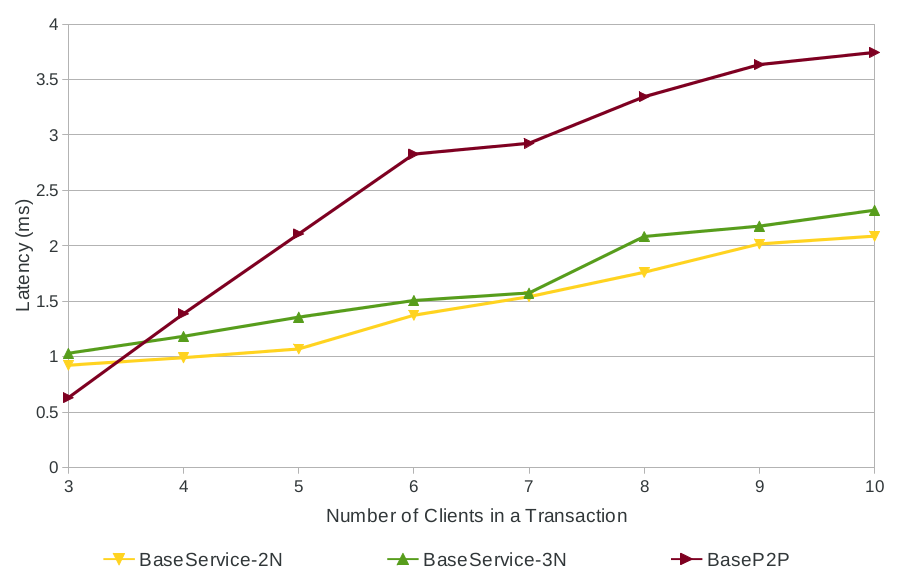
\includegraphics[width=\textwidth,height=\textheight,keepaspectratio]{latency}
 \caption{Comparison of Latency}
 \label{fig:LatencyGraph}
\end{figure}

\begin{figure}[htbp!]
% \centering
 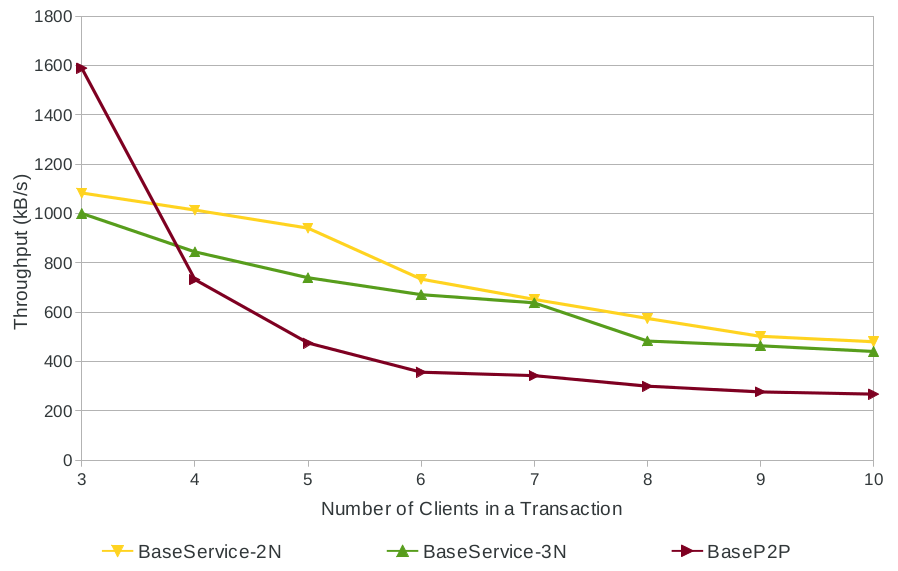
\includegraphics[width=\textwidth,height=\textheight,keepaspectratio]{throughput}
 \caption{Comparison of Throughput}
 \label{fig:ThroughputGraph}
\end{figure}

Figures \ref{fig:LatencyGraph} and \ref{fig:ThroughputGraph} show latency and throughput, with $2N$ and $3N$ denoting $n=2$ and $n=3$. Each plot on the graph is an average of 3 \emph{crash-free} trials; a trial consists of each $c$ node completing $10^4$ transactions for a specific value of $|T_x.dst|$. Thus, BaseService receive a total of $10^5$ \emph{abcast} requests in each trial. In BaseP2P, each $c$ node initiates $10^4$ Base executions with its peers and the steady throughput in Figure \ref{fig:ThroughputGraph} as $|T_x.dst| \rightarrow 10$ suggests an absence of node saturation.

Referring to Fig \ref{fig:LatencyGraph}, as $|T_x.dst| \geq 4$, BaseP2P's \emph{abcast} latencies increase considerably, indicating that \emph{abcast} is best provided as a service for scalable performance. Comparing throughput in Figure \ref{fig:ThroughputGraph} leads to similar conclusions.

\noindent \textbf{Summary}: \emph{Abcast}ing is best offered as a service to a large-scale distributed transaction system. 

\section{Limitations of Existing Atomic Broadcast Solutions}
Section \ref{sec:abaas_results} clearly shows that transaction throughput can be improved by utilising the \textsf{AbaaS} model for \emph{abcast} ordering.  However, the existing protocol used, TOA, is a GM based protocol that blocks severely when node crashes occur.  This blocking behaviour is acceptable when TOA is utilised between client nodes, as it is presumed that blocking will only occur at a small subset of the overall cluster, thus system \emph{liveness} still exists in the majority of the cluster.  However, if all $s$-nodes utilise TOA for \emph{abcast}ing and a single $s$-node crashes, all $s$-nodes will block, resulting in no client requests being satisfied. Therefore, not only are the $s$-nodes blocked, but as a consequence of this blocking, so is the entire cluster.  Thus the entire system's \emph{liveness} is lost until the GM protocol detects the $s$-node crash and unblocks the ordering service.  GM based protocols, such as TOA, cannot be used as the basis of a \textsf{AbaaS} service as system-wide blocking would be catastrophic for any in-memory database.  

As detailed in sections \ref{sec:limitations_existing_coordination} and \ref{sec:coordination}, quorum based \emph{abcast} protocols are not suitable for use in \textsf{AbaaS} due to their tendency to block mildly when the master is falsely/validly suspected of crashing, and because of the performance limitations associated with master based protocols.  

Therefore, in order for \textsf{AbaaS} to be valid system model, a new \emph{abcast} protocol is required.  The \emph{abcast} protocol must allow for low-latency, high-throughput \emph{abcast}s, as provided by GM based protocols, in addition to providing non-blocking behaviour in the presence of node failures.  